\documentclass[bigger]{beamer}

\mode<presentation>{
  \usetheme{default}
  \usefonttheme{serif}
  \setbeamercovered{transparent}
  \setbeamerfont{institute}{size=\footnotesize}
}

\usepackage[english]{babel}
\usepackage{times}
\usepackage{algorithmic}
\usepackage{algorithm}

% Latin-1 only
\usepackage[latin1]{inputenc}
\usepackage[T1]{fontenc}
%--------------------------------------------------
% % Chinese-support
% \usepackage[nocjkbg5]{ucs}
% \usepackage[utf8x]{inputenc}
% \usepackage[C00,T1]{fontenc}
% \newcommand\tradtext[1]{\bgroup\fontencoding{C00}\fontfamily{ming}\selectfont%
% \SetUnicodeOption{cjkbg5}#1\egroup}
%-------------------------------------------------- 

\title[]{Survey: Organizing and Searching the World Wide Web of Facts}
\author[]{Ruey-Cheng Chen} 
\institute{Academia Sinica, Taiwan}
\date[]{}
\subject{Theoretical Computer Science}
%--------------------------------------------------
% \AtBeginSubsection[]
% {
%   \begin{frame}<beamer>
%     \frametitle{Outline}
%     \tableofcontents[currentsection,currentsubsection]
%   \end{frame}
% }
%-------------------------------------------------- 
%\beamerdefaultoverlayspecification{<+->}
\newcommand<>\ul[2]{\textbf{#1}\begin{itemize}#2\end{itemize}}
\newcommand<>\ull[1]{\begin{itemize}#1\end{itemize}}
\newcommand<>\ol[2]{\textbf{#1}\begin{enumerate}#2\end{enumerate}}
\newcommand<>\dl[2]{\textbf{#1}\begin{description}#2\end{description}}

\newcommand<>\f[2]{\begin{frame}{#1}#2\end{frame}}
%--------------------------------------------------
% \newcommand\slide[1][]{\begin{frame}{#1}}
%-------------------------------------------------- 

\begin{document}

\frame{ \titlepage }

\f{References}{

  \ul{Mandatory Reference}{ \item M. Pa\c sca, D. Lin, J. Bigham, A. Lifchits,
  and A. Jain. Organizing and Searching the World Wide Web of Facts -- Step
  One: the One-Million Fact Extraction Challenge.  AAAI'06.  \item M. Pa\c sca.
  Organizing and Searching the World Wide Web of Facts -- Step Two: Harnessing
  the Wisdom of the Crowds.  WWW'07.  }

  \ul{Authors}{\item Marius Pa\c sca:
  \footnotesize{\url{http://research.google.com/pubs/author107.html}} \item
  Dekang Lin \footnotesize{\url{http://www.cs.ualberta.ca/~lindek/}}}

}

\f{Outline}{ \tableofcontents }

\section{Step One: Large-Scale Fact Extraction from the Web}

\subsection{Contextual Extraction Patterns}
\f{Basic Contextual Extraction Patterns}{

  \ul{Seed Facts}{ \item The pair of phrases that are in a ``hidden'' relation
  \ull{ \item Person-BornIn-Year: (\emph{Vincenzo Bellini},
  \emph{1801}), City-CapitalOf-Country: (\emph{Athens}, \emph{Greece}),
  Language-SpokenIn-Country: (\emph{Portuguese}, \emph{Brazil})} }

  \ul{Contextual Extraction Patterns}{ \item Template: <prefix> A <infix> B
  <postfix> \ull{ \item ``\emph{The proposed trip will take students to
  \alert{Athens}, the capital of \alert{Greece} and home to 40\% of the Greek
  population}'' } \item Trie-based on top of MapReduce \cite{dean2004msd} }

}

\f{Generalization via Distributionally Similar Words}{

  \begin{columns}[t]
    \begin{column}{5cm}

      \ul{Generalized Patterns}{ \item Terms in the \{pre,in,post\}fix replaced
      with classes \cite{lin1998ara} (extracted from 50 million news articles)
      \item Digits replaced with markers ``0'' \item Patterns enumerated
      exhaustively (discarding ones with bogus infix)}

    \end{column}
    \begin{column}{7cm}

      \begin{figure} 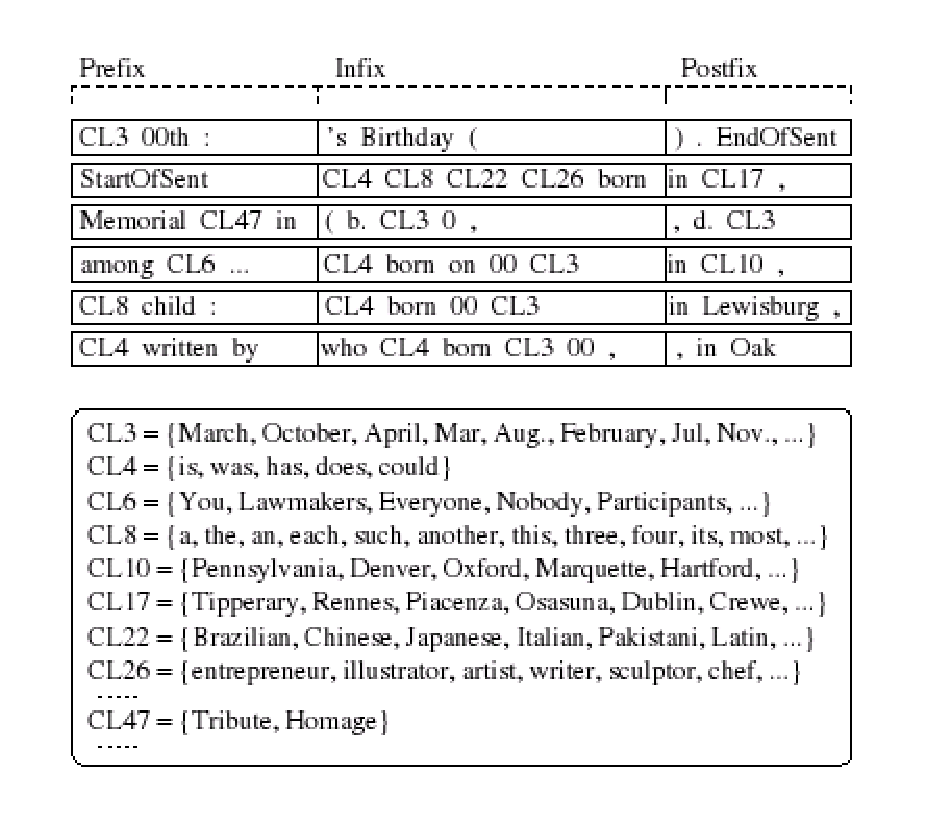
\includegraphics[width=\columnwidth]{step1/fig1.eps} \end{figure}

    \end{column}
  \end{columns}
}

\f{Validation and Ranking Criteria}{

  \ul{Populating Candidates}{ \item The end of prefix and the start of postfix \item
  Higher recall approximation: loose matching of the POS tags around the facts and infix }

  \ul{Validating Candidates}{ \item Distributional similarity-based method
  \item e.g. A known fact (\emph{Stephen Foster}, \emph{1826}) \ull{ \item
  (\emph{Robert S. McNamara}, \emph{1826}) => OK \item (\emph{Web Page},
  \emph{1989}) => \alert{DISCARDED} } }

  \ul{Ranking}{ \item PMI-inspired score \cite{turney2001mws} \item Completeness score }

}

\subsection{Evaluation}
\f{Experimental Setting}{

  \ul{Text Collection}{ \item Web snapshot taken in 2003 by Google \item Three
  chunks $W_1$, $W_2$, and $W_3$ (each sized 100 million docs.) }
  \ul{Target Facts}{ \item Person-BornIn-Year (due to its high availability on the Web) }
  \ul{Seed Set}{ \item 10 randomly selected seed facts }

  \begin{small}
    \begin{tabular}{|ll|}
      \hline
      (\emph{Irving Berlin}, \emph{1888}) & (\emph{Hoagy Carmichael}, \emph{1899}) \\
      (\emph{Bob Dylan}, \emph{1941}) & (\emph{Stephen Foster}, \emph{1826}) \\
      (\emph{John Lennon}, \emph{1940}) & (\emph{Paul McCartney}, \emph{1942}) \\
      (\emph{Johann Sebastian Bach}, \emph{1685}) & (\emph{Bela Bartok}, \emph{1881}) \\
      (\emph{Ludwig van Beethoven}, \emph{1770}) & (\emph{Vincenzo Bellini}, \emph{1801}) \\
      \hline
    \end{tabular}
  \end{small}
}

\f{Evaluation: Quantitative Results}{
  \textbf{Unique Names Extracted by Patterns}
  \begin{figure}
  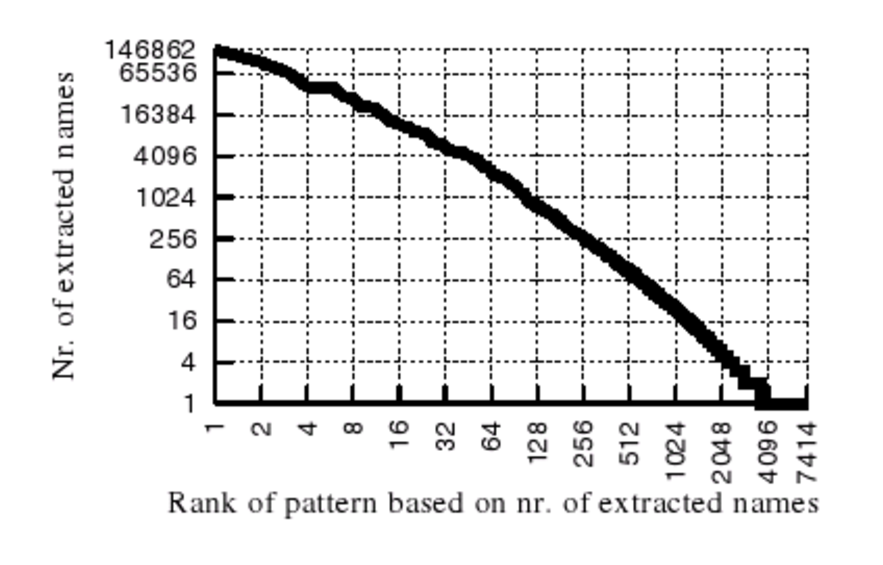
\includegraphics[width=250pt]{step1/fig2.eps}
  \end{figure}
}

\f{Evaluation: Quantitative Results (cont'd)}{
  \textbf{Unique Names Extracted by Hosts}
  \begin{figure}
  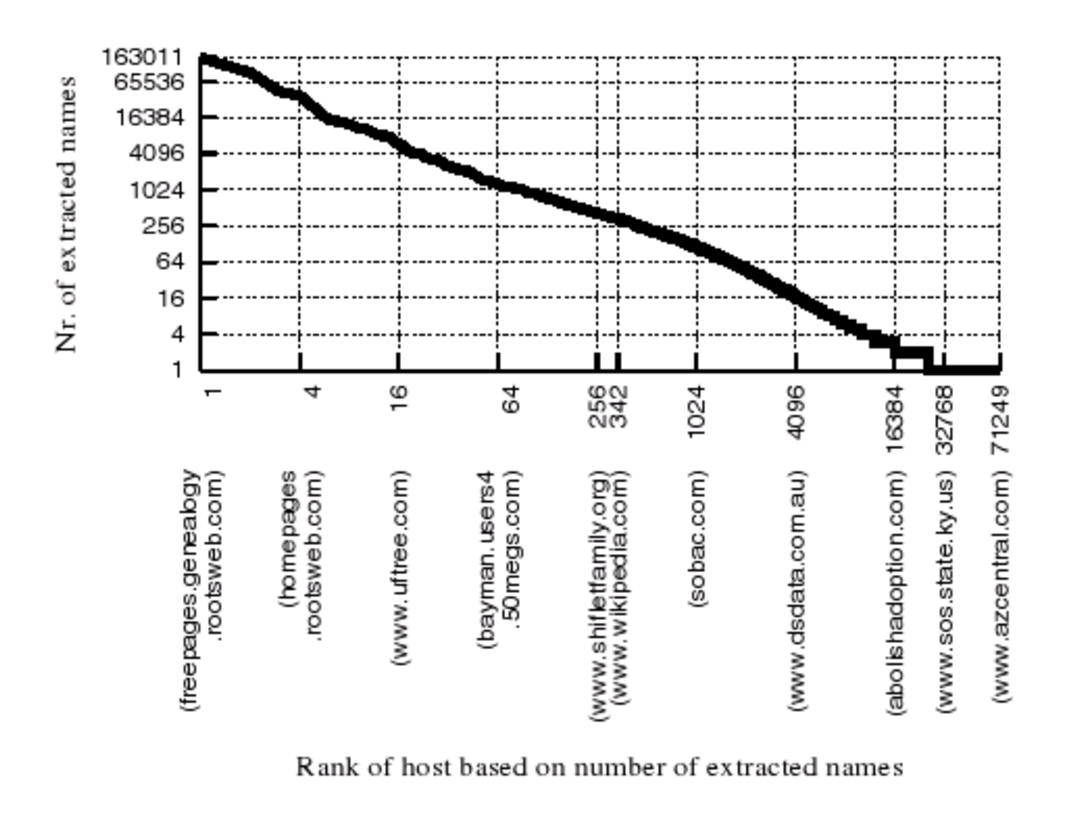
\includegraphics[width=250pt]{step1/fig3.eps}
  \end{figure}
}

\f{Evaluation: Accuracy of the Extracted Facts}{

  \ul{Evaluation}{\item Sample Set: $W_1$ divided into 10 subsets \item Manual
  assessment (based on supporting evidence)}
 
  \begin{figure}
  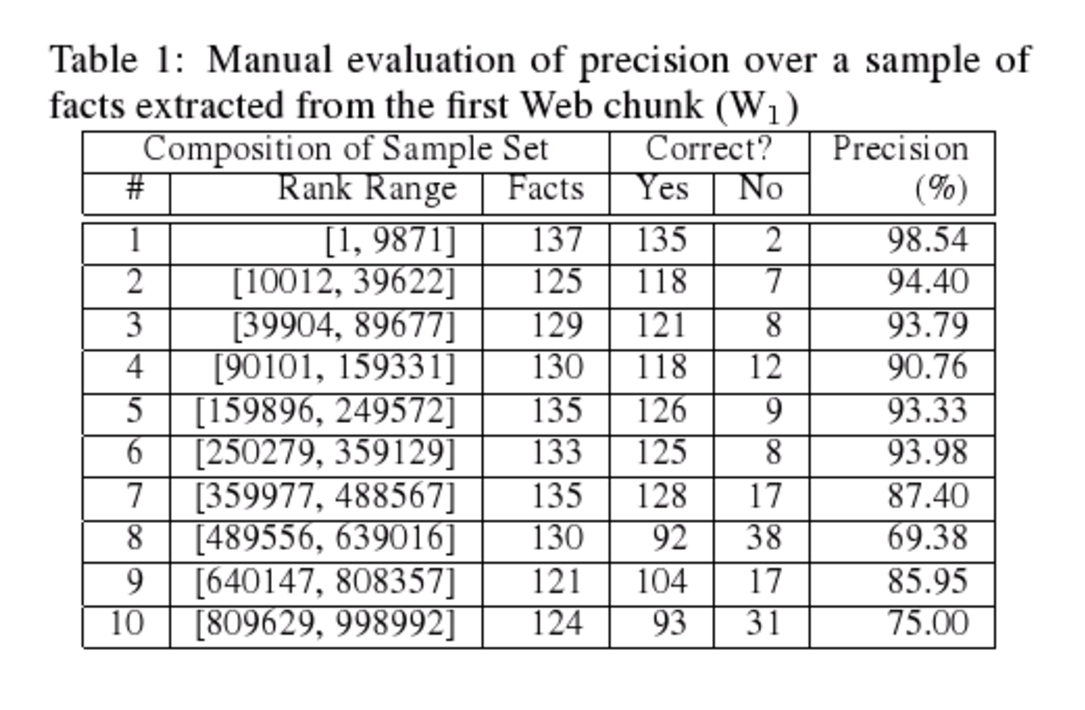
\includegraphics[width=250pt]{step1/tbl1.eps}
  \end{figure}
}

\f{Evaluation: Coverage of the Extracted Facts}{

  \ul{Evaluation}{\item Gold Standard: random selection of 6,617 pairs from
  Wikipedia \item Automatic \ull{\item MRR score $\frac{1}{Rank}$ } }
 
  \begin{figure}
  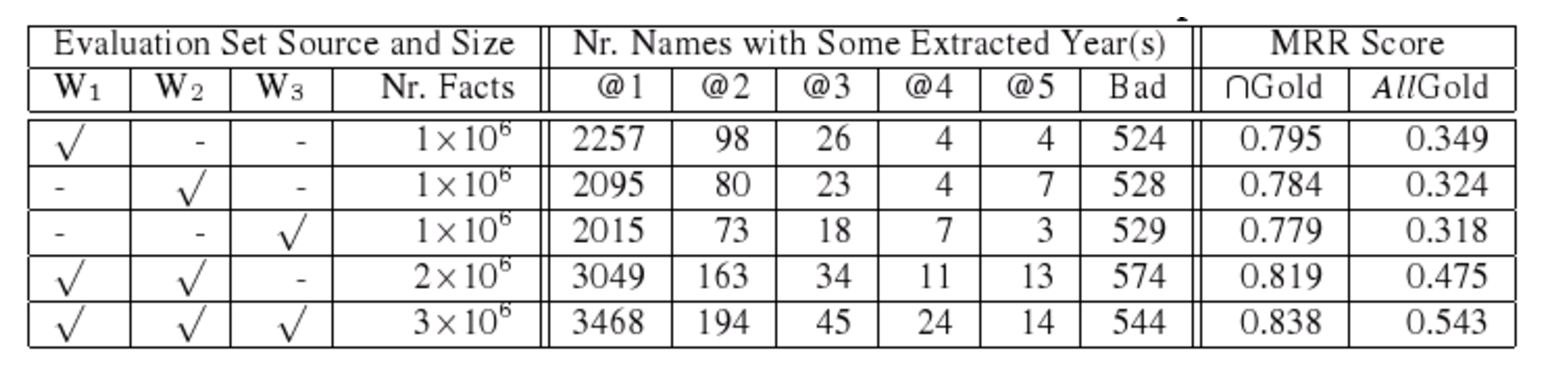
\includegraphics[width=250pt]{step1/tbl2.eps}
  \end{figure}
}

\section{Step Two: Fact Extraction from Search Queries}

\subsection{Weakly Supervised Extraction Framework}
\f{Weakly Supervised Extraction Framework}{

  \ul{Input}{ \item Target class $C$, available as a set of instances $\{I\}$
  \item Small set of seed phrases $\{K\}$ expected in output \item Large
  repository of search queryies $\{Q\}$ }

  \ul{Output}{ \item A ranked list of phrases for $C$ }

  \ul{Steps}{ \item Collecting a pool of phrases $\{P\}$ \item For each
  search signature $(P, I)$ and $Q$ containing both $P$ and $I$, populating
  template and updating its frequency \item Merge templates for seed phrases
  \item Ranking each $P$ according to its similarity to the reference templates
  }

}

\f{Algorithm}{
  \begin{figure} 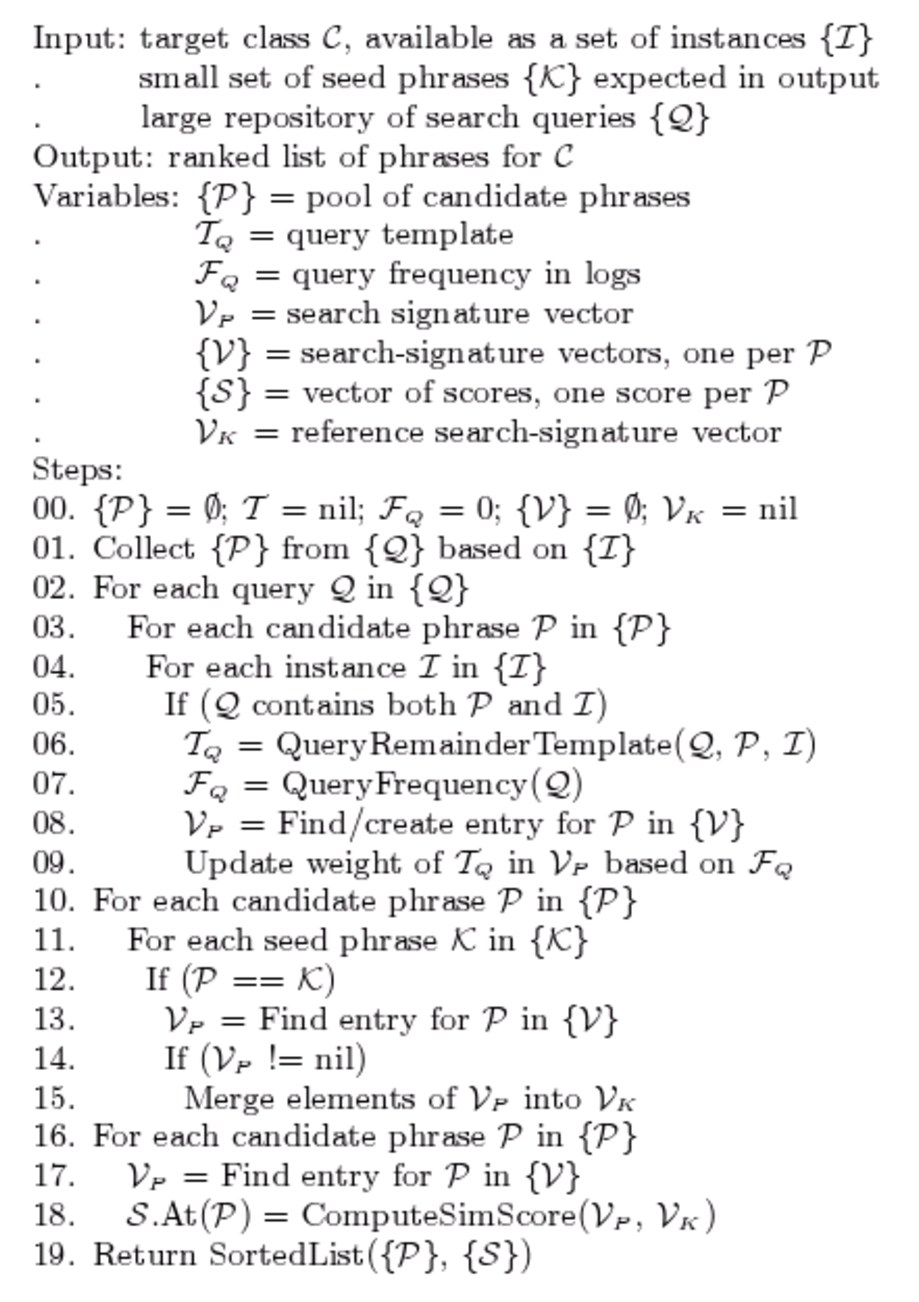
\includegraphics[width=160pt]{step2/fig1.eps} \end{figure}
}

\f{Overview of the Framework}{
  \begin{figure} 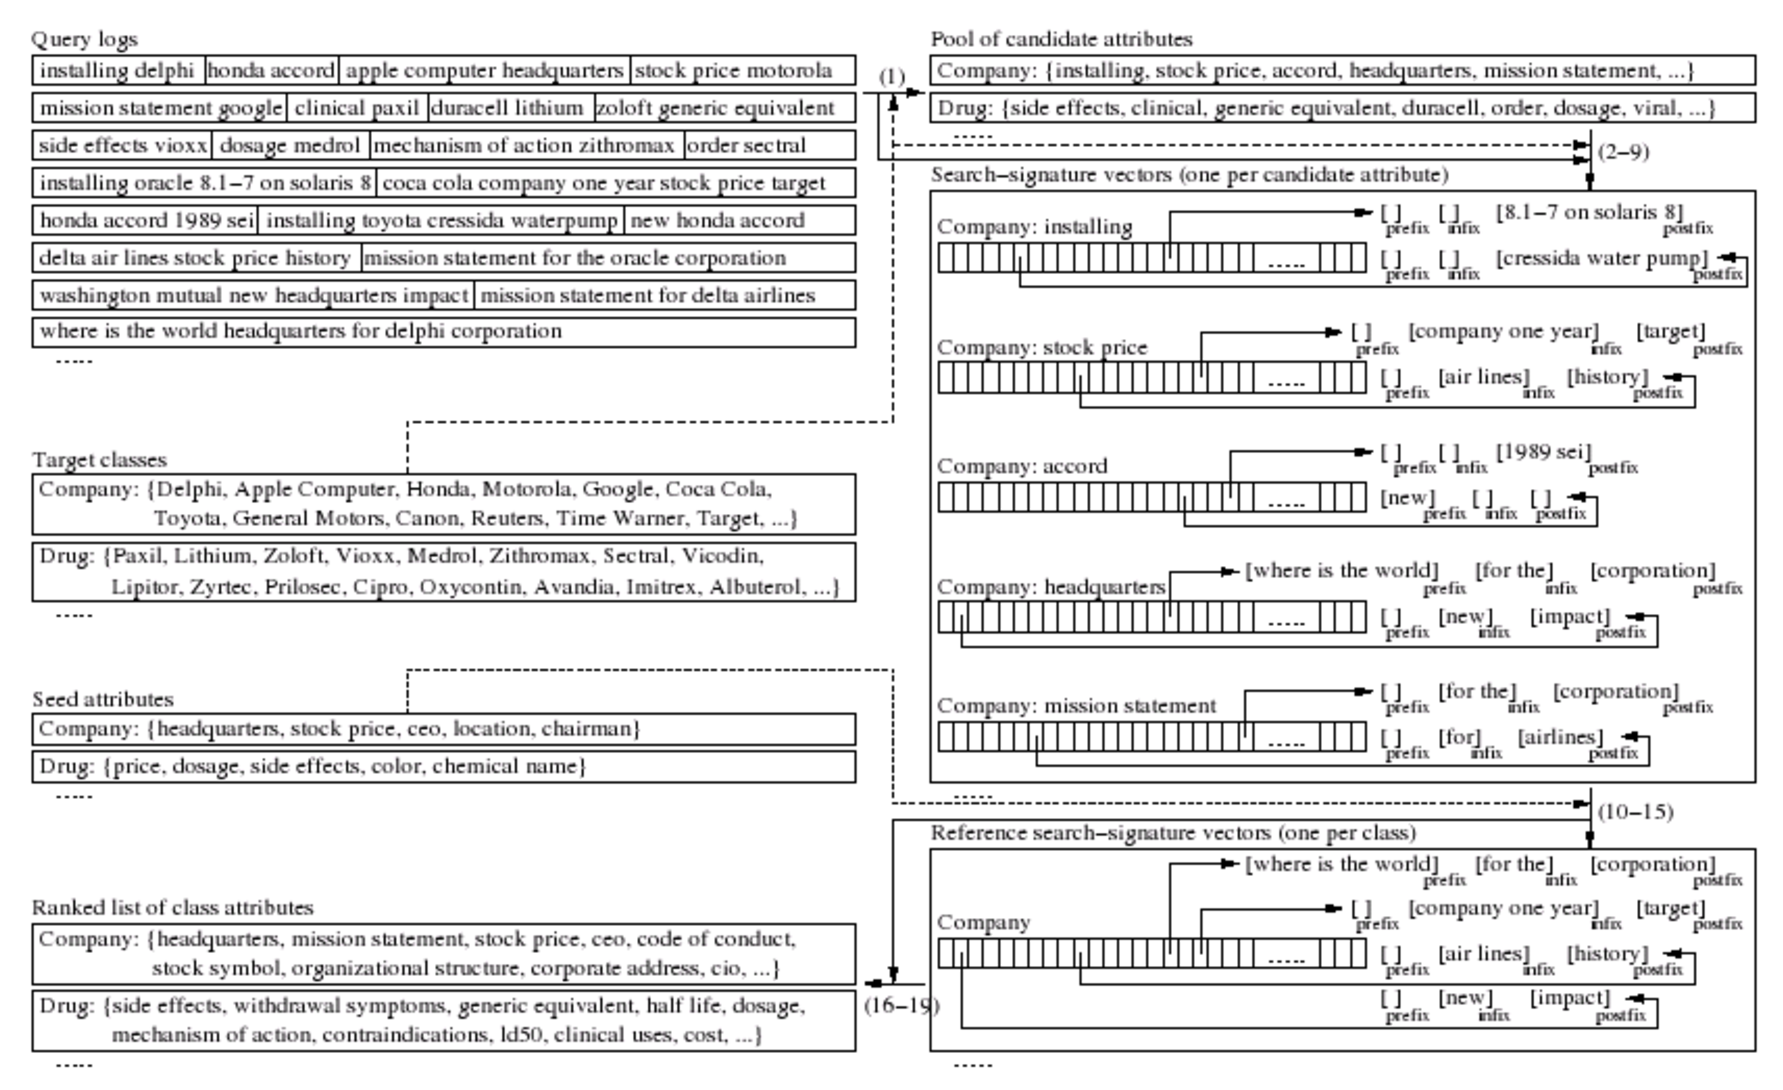
\includegraphics[width=\columnwidth]{step2/fig2.eps} \end{figure}
}

\subsection{Evaluation}
\f{Experimental Setup: Data}{
  \textbf{Percentage of input queries of various lengths}
  \begin{figure}
  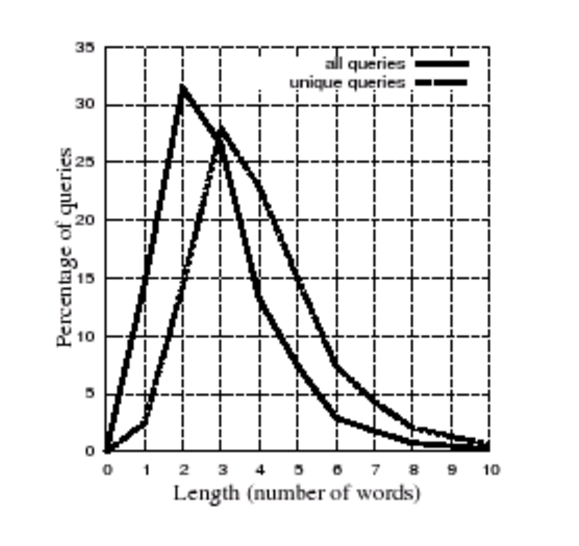
\includegraphics[width=200pt]{step2/fig3.eps}
  \end{figure}
}

\f{Experimental Setup: Target Classes}{
  \begin{figure}
  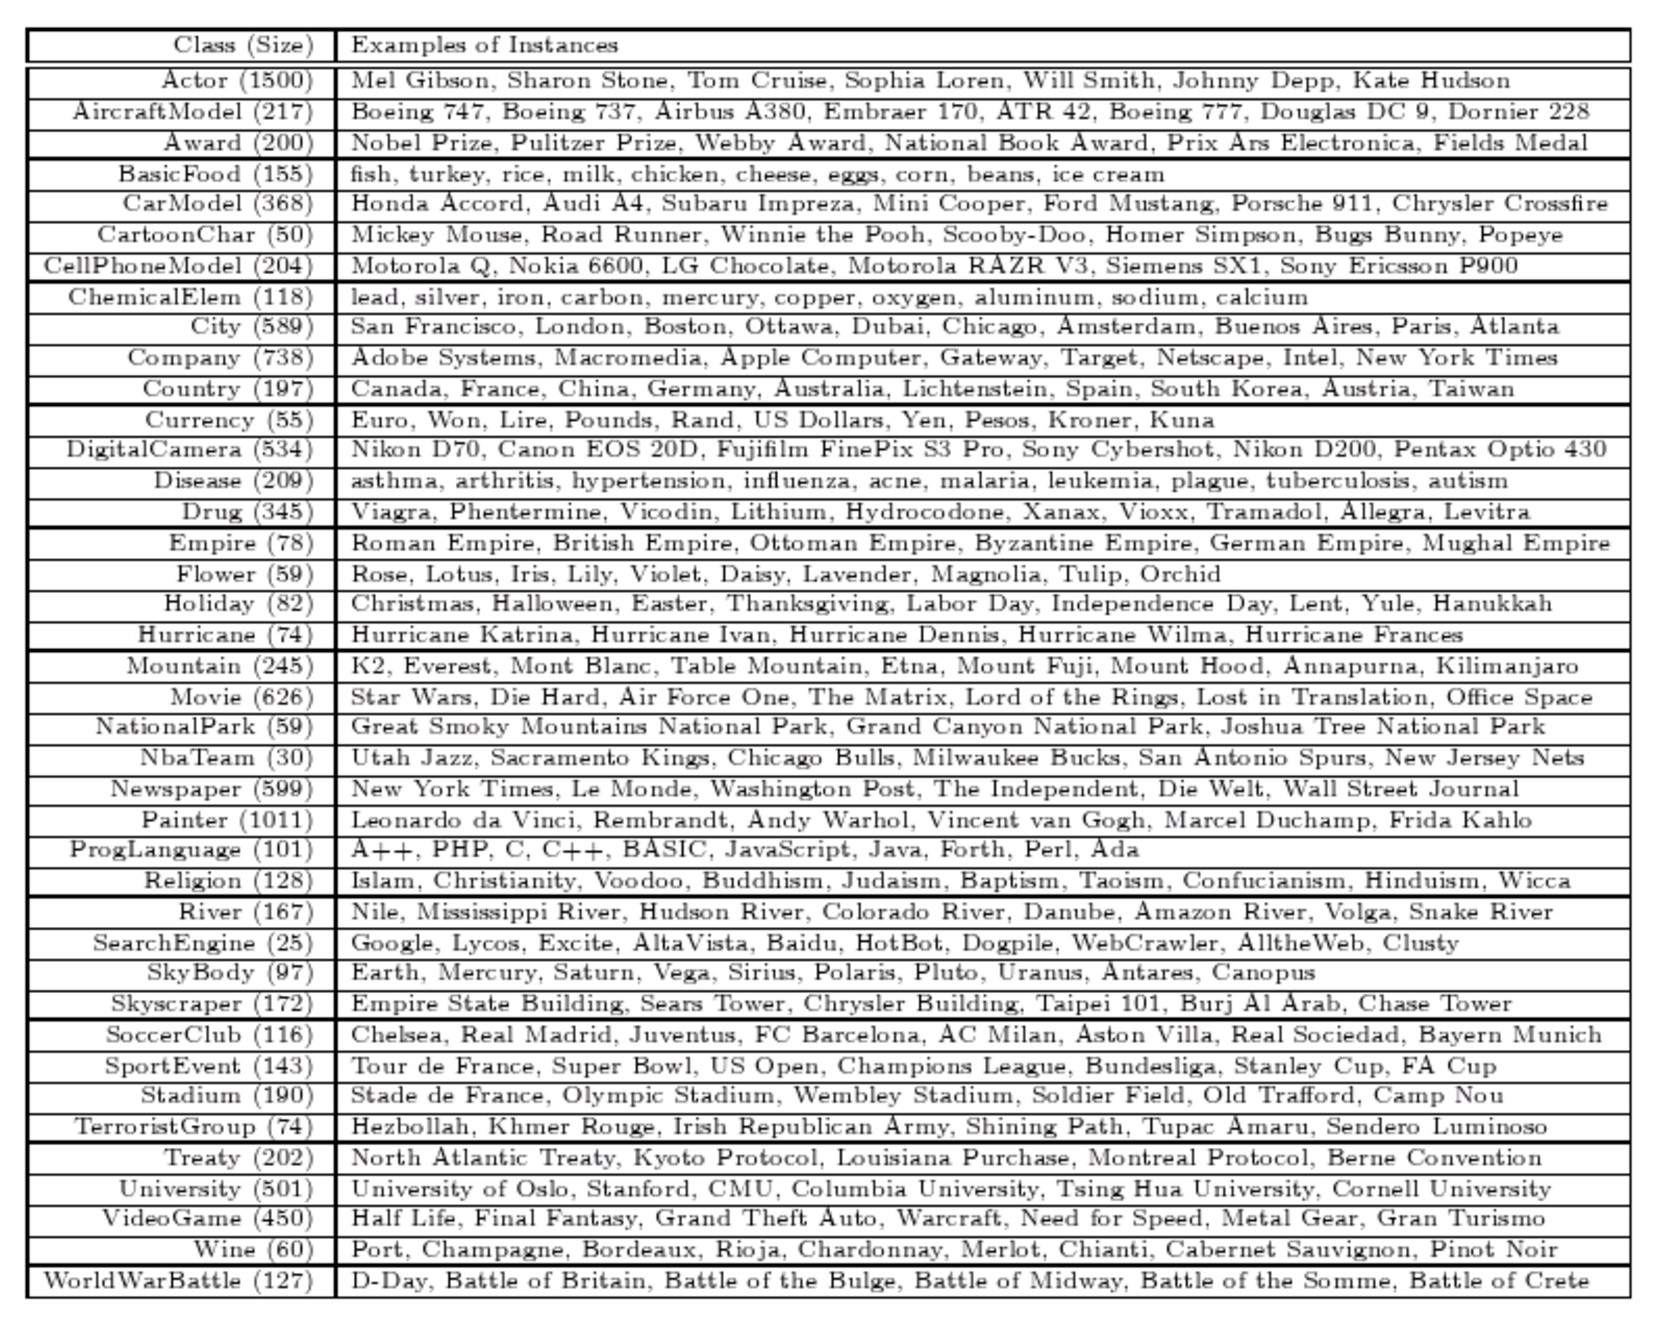
\includegraphics[width=250pt]{step2/tbl1.eps}
  \end{figure}
}

\f{Experimental Setup: The Rest}{

  \ul{Evaluation}{\item Seed attributes: 5 for each target class, independently
  chosen (e.g. \{\emph{quality}, \emph{speed}, \emph{number of
  users}, \emph{market share}, \emph{reliability}\} for \emph{SearchEngine})
  \item Similarity Functions \ull{ \item Cosine \item JS-divergence \item
  L1-Norm \item Skew-Divergence} \item Task: class attribute extraction, manual assessment (\emph{vital}, \emph{okay}, \emph{wrong})}

  \begin{figure}
  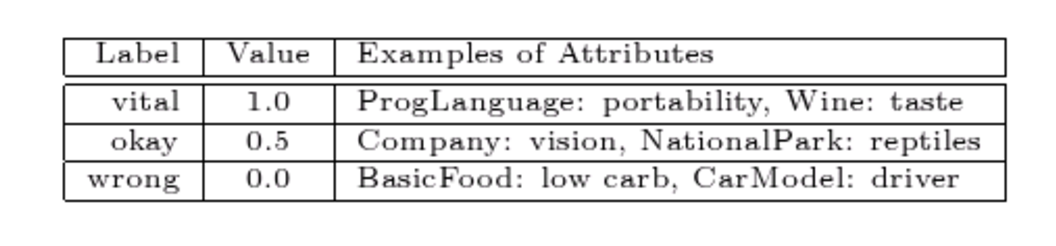
\includegraphics[width=200pt]{step2/tbl2.eps}
  \end{figure}
}

\f{Evaluation: Performance}{
  \begin{figure}
  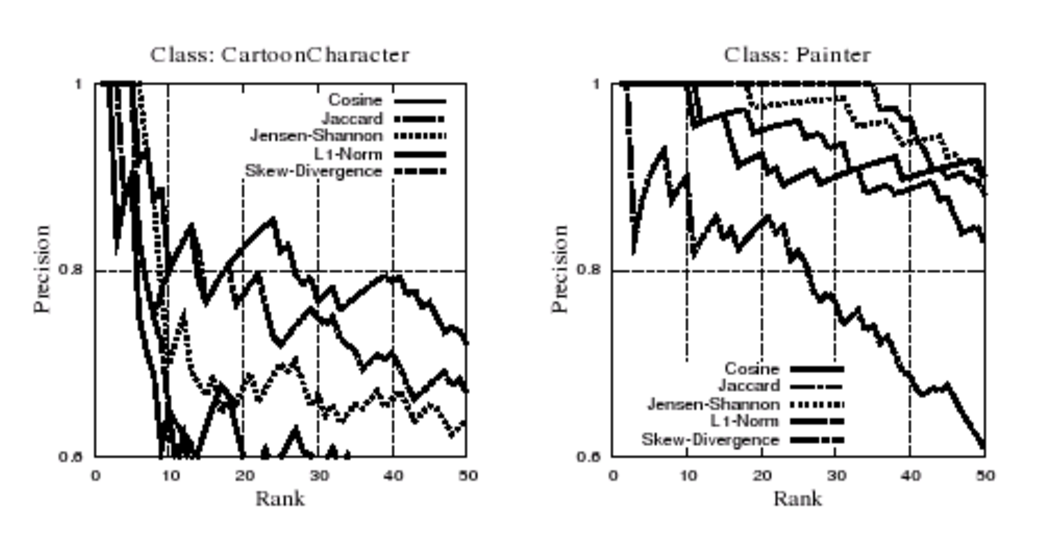
\includegraphics[width=\columnwidth]{step2/fig4-1.eps}
  \end{figure}
}

\f{Evaluation: Performance (cont'd)}{
  \begin{figure}
  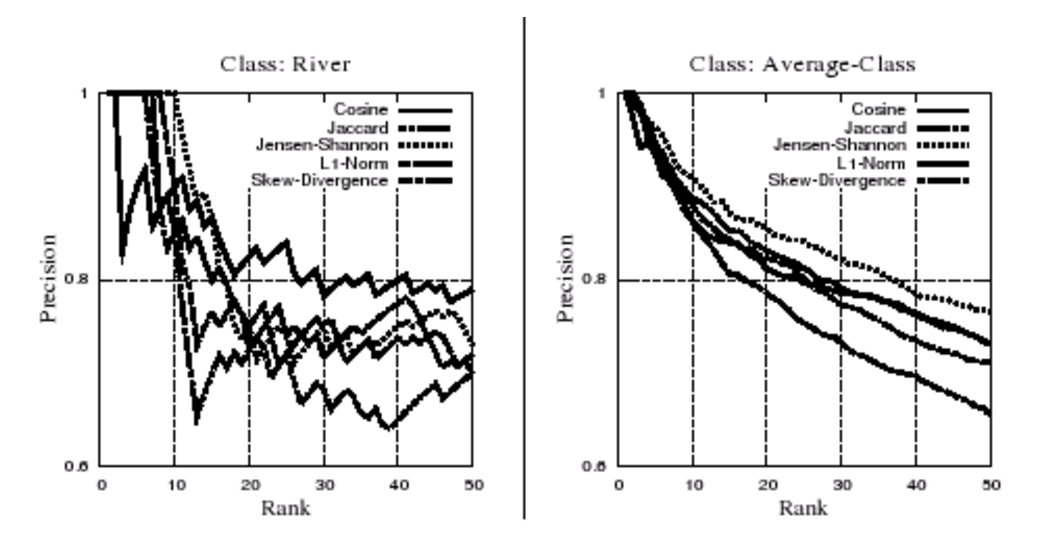
\includegraphics[width=\columnwidth]{step2/fig4-2.eps}
  \end{figure}
}

\f{Evaluation: Top Attributes}{
  \begin{figure}
  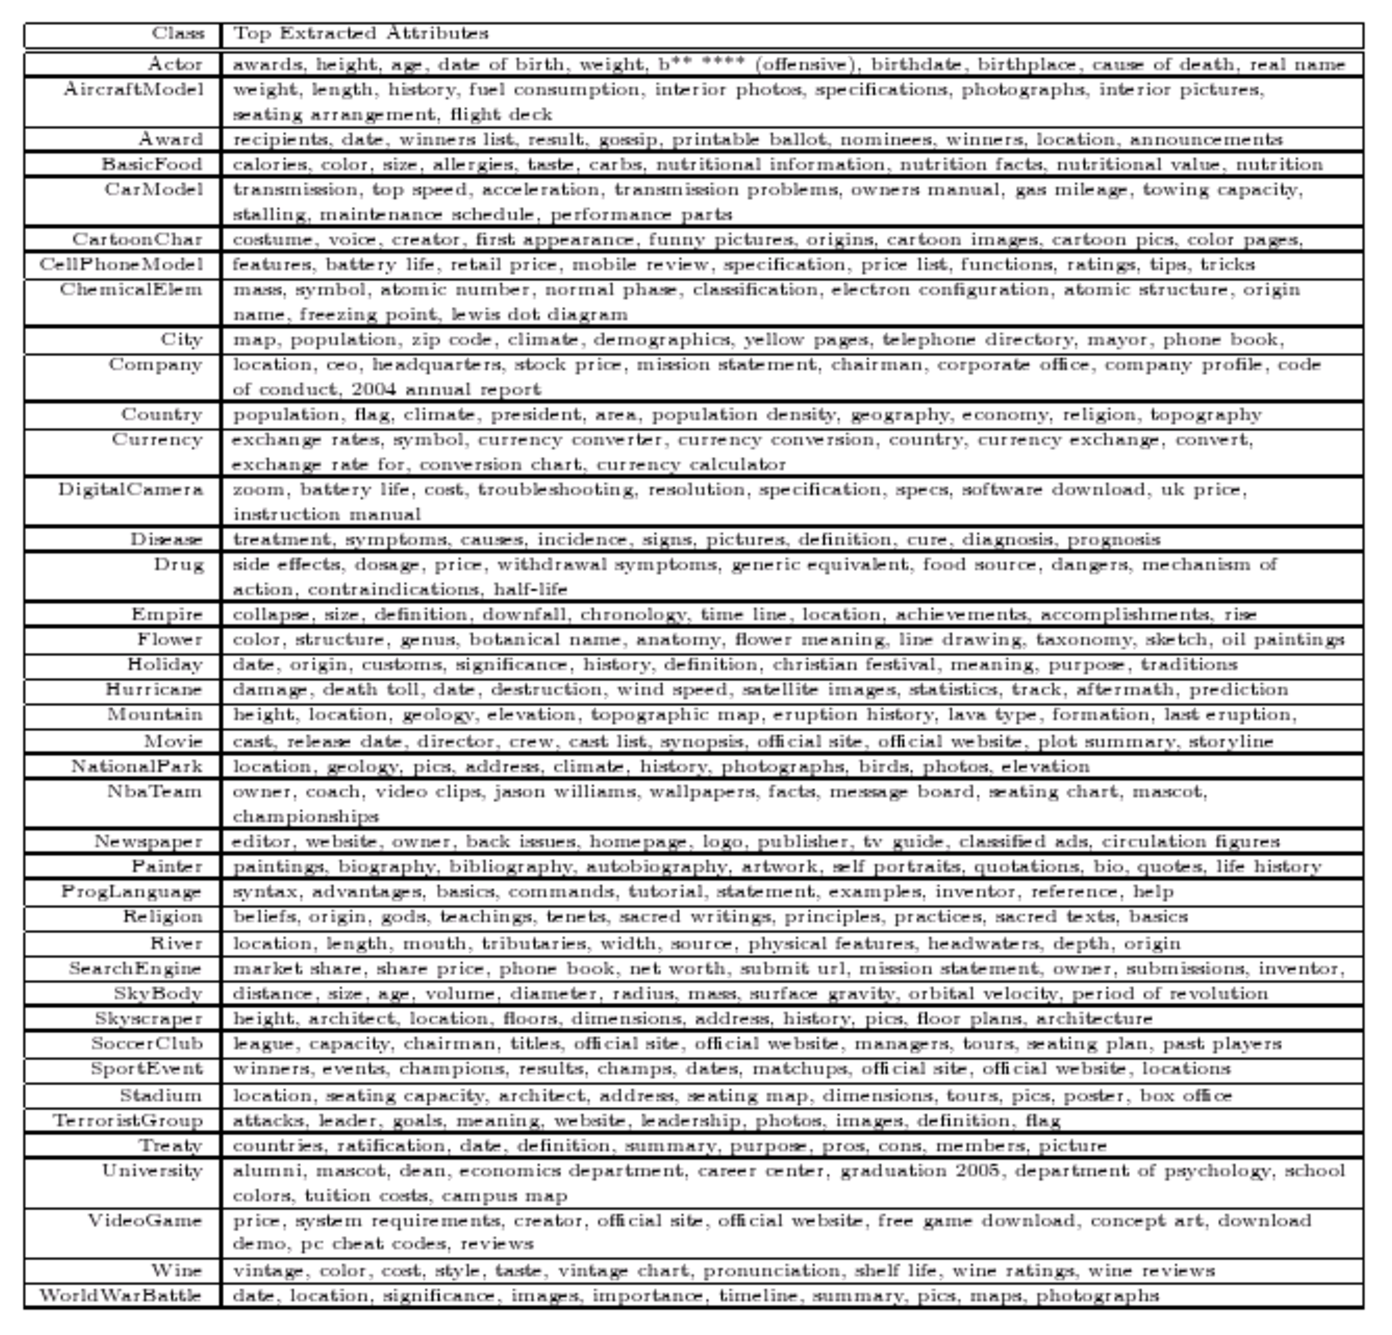
\includegraphics[width=250pt]{step2/tbl3.eps}
  \end{figure}
}

\f{Evaluation: Comparison}{
  \begin{figure}
  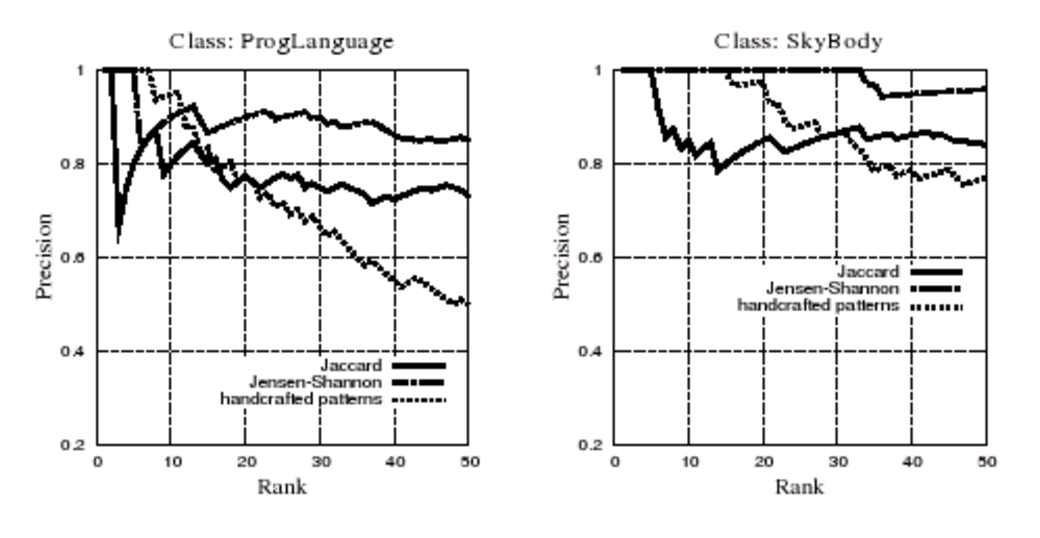
\includegraphics[width=\columnwidth]{step2/fig5-1.eps}
  \end{figure}
}

\f{Evaluation: Comparison (cont'd)}{
  \begin{figure}
  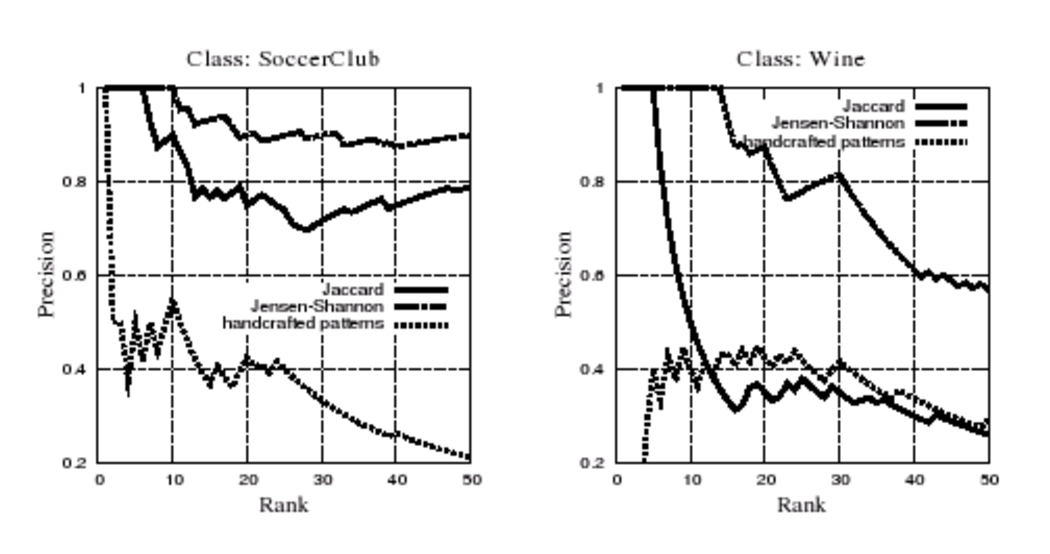
\includegraphics[width=\columnwidth]{step2/fig5-2.eps}
  \end{figure}
}

\f{Evaluation: Detailed Comparison}{
  \ul{Methods}{\item $P_{old}$ (handcrafted patterns) vs. $S_{new}$ (seed-based extraction with JS-divergence)}
  \begin{figure}
  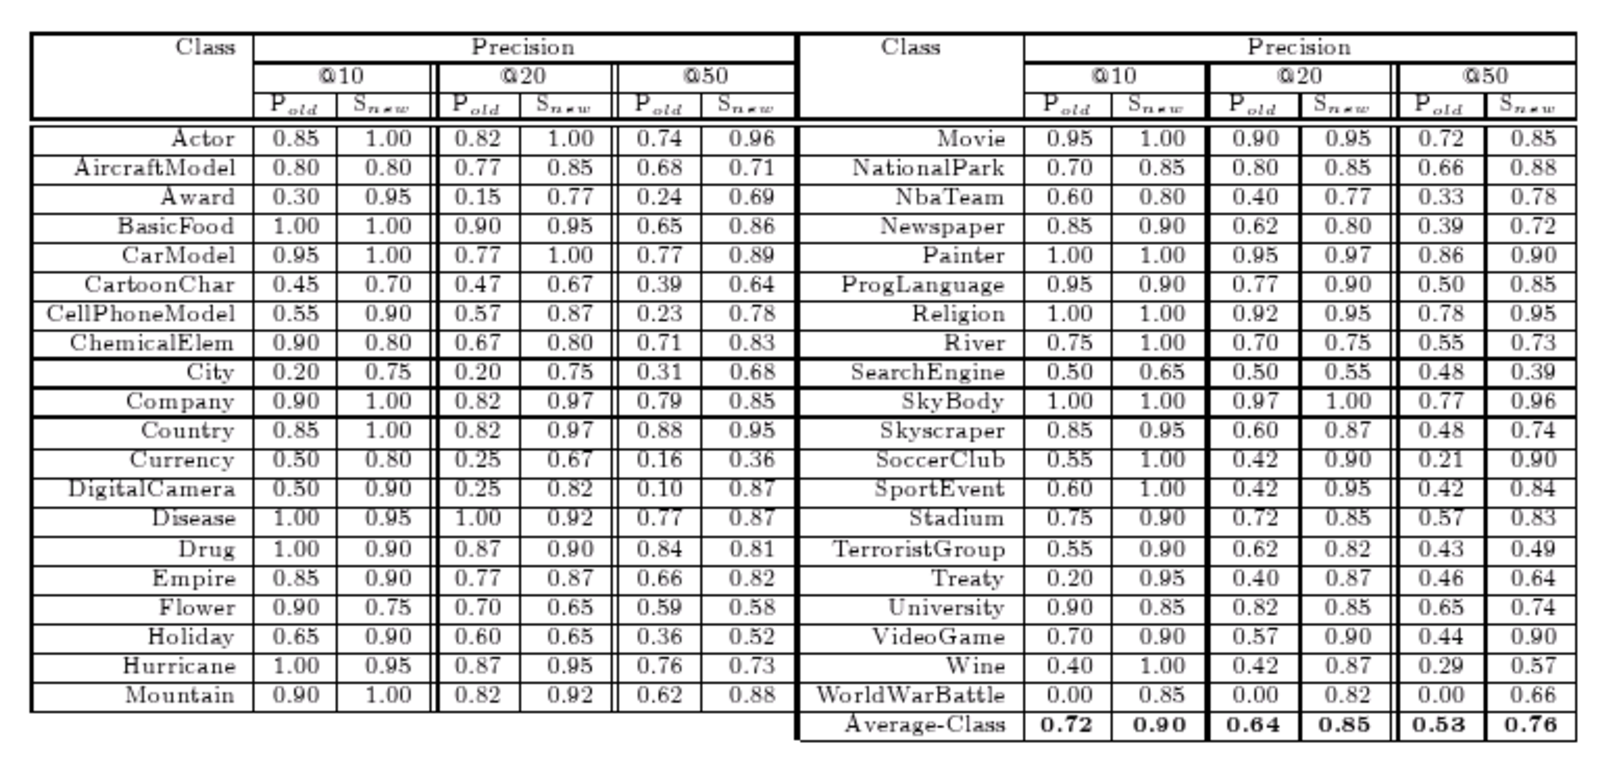
\includegraphics[width=\columnwidth]{step2/tbl4.eps}
  \end{figure}
}

\subsection{Minimizing the Amount of Supervision}
\f{Minimizing the Amount of Supervision}{
  \ul{Evaluation}{\item Varying the number of instances and the number of seeds per class}
  \begin{figure}
  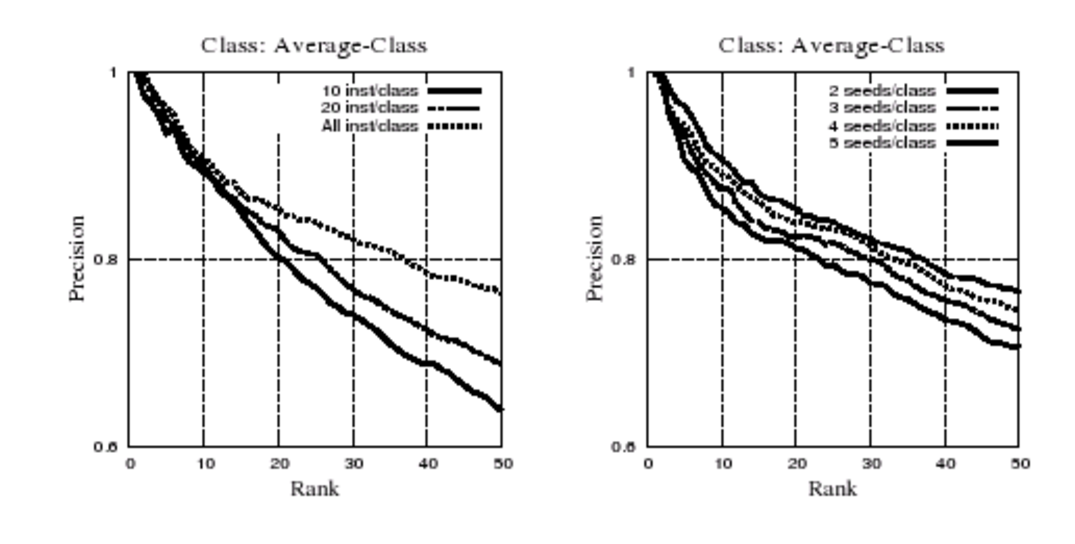
\includegraphics[width=250pt]{step2/fig6.eps}
  \end{figure}
}

\subsection{Identifying Near-Duplicate Attributes}
\f{Identifying (Near-Duplicate) Attributes}{
  \begin{figure}
  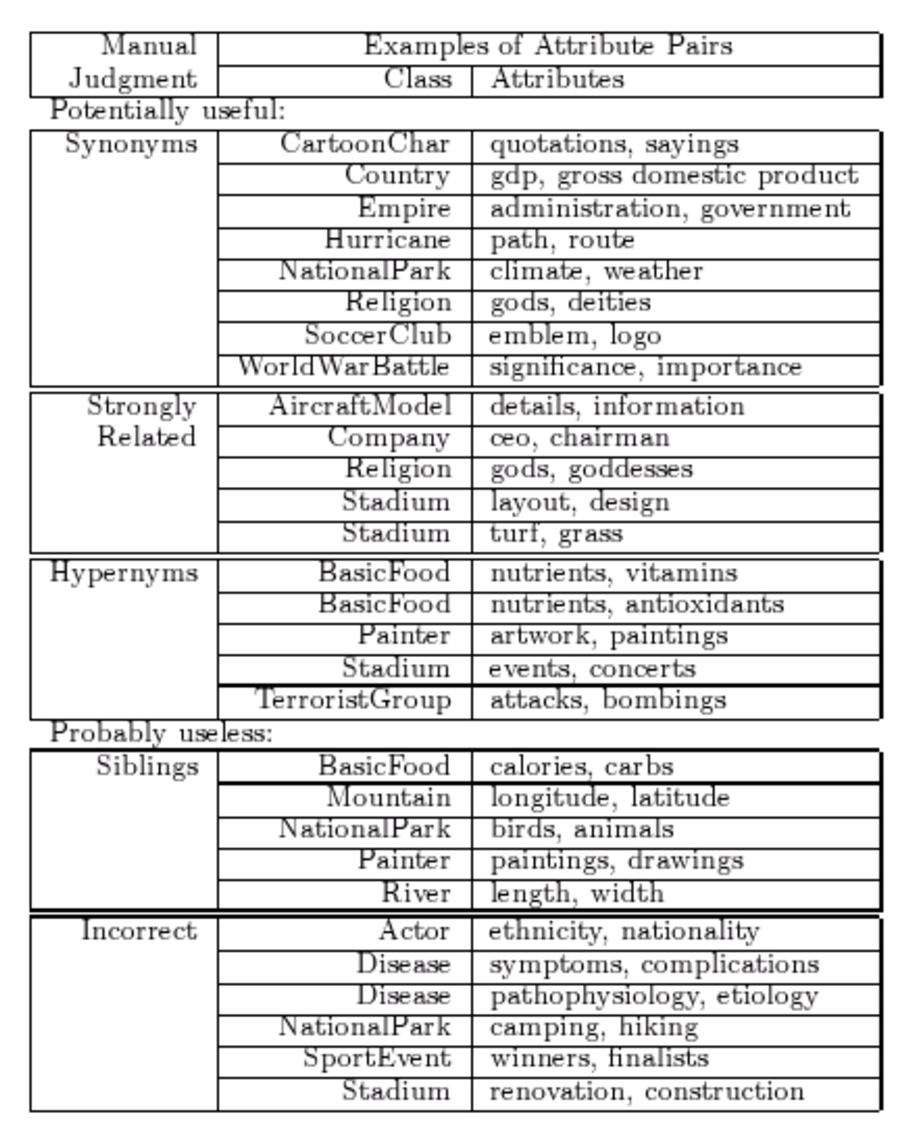
\includegraphics[width=180pt]{step2/tbl5.eps}
  \end{figure}
}

\section{Conclusions}
\f{Conclusions}{
  \ul{Step One}{ \item Automatic approach \item Approximately 90\% precision over 100 million Web docs.}
  \ul{Step Two}{ \item Weakly-supervised extraction framework for query log mining \item Outperforming previous methods \item Extensive study}
}

\section<presentation>*{\appendixname}

\begin{frame}%[allowframebreaks]
  \frametitle{References}
  \small
  \bibliography{report}
  \bibliographystyle{alpha}
\end{frame}

\frame{
  \begin{center}
    \Huge{Thanks for your attention!}
    \par
    Any Question?
  \end{center}
}

\end{document}
